\newpage %! newpage
\chapter{Analyse der erhobenen Daten}


% ------------------------------------------- Lizenzen ------------------------------------------- %
\section{Lizenzen}

\todo{Verweis auf Kapitel 2.1 Lizenzen => Warum genau diese Aufteilung}

\todo{Bonus Formulierung: Die Projekte die offen sind befinden sich in den Top 50\%....}

\bigskip
\noindent
Zunächst wurden die Datensätze in zwei Gruppen aufgeteilt, Projekte mit freizügigen und restriktiven
Lizenzen. \todoo{Die Aufteilung erfolgt hierbei wie im Kapitel 1.3.3.7 zu Lizenzen näher erklärt wurde.}
In der Tabelle \ref{tab:lizenzen} findet sich eine Zusammenfassung aller Lizenzen der
Projekte die erfasst worden sind. Wie man erkennt haben 91\% der Projekte eine freizügige Lizenz, wobei
die MIT Lizenz mit 69\% die beliebteste aller Lizenzen ist. Um die Beliebtheit der Projekte zu
vergleichen wurden die GitHub Sterne als Metrik verwendet.
Aufgrund der stark ungleich großen Gruppen wurden anhand von Gruppen anhand von Ranking verglichen.
Hierfür wurden die Projekte, wie in Abbildung \ref{abb:permissive_vs_restriktiv_BarChart} zu sehen
ist, absteigend nach Anzahl der Sterne sortiert.
Das erste Projekt mit einer restriktive Lizenz belegt hierbei den Platz 35. Projekte mit freizügige
Lizenzen übertreffen die restriktiven sowohl in der Menge als auch in ihrer Beliebtheit.
%
%
%
% Daten von GitHub
% In 2015 hat GitHub in einem Blogeintrag die Aufteilung der Lizenznutzung auf ihrer Platform veröffentlicht
% \cite{OpenSourceLicense2015}. Wie man in Tabelle \ref{tab:GitHub_Blog_Lizenznutzung2015} sehen kann,
% haben 64\% aller Projekte permissive Lizenzen und 24\% restriktive. 15\% der Projekte haben keine
% Standardlizenz und werden von GitHub daher als \textit{other} kategorisiert.
%
%
% \subsubsection*{Anmerkung:}
% Die Tabelle \ref{tab:GitHub_Blog_Lizenznutzung2015} ergibt in der Summe über 100\%. Grund hierfür
% könnte sein, dass einige Projekte Dual Lizenzen besitzen
%
% H1 Bestätigt sich.
Somit bestätigt sich die \hyperref[H:1]{Hypothese H1}. Projekte mit freizügigen Lizenzen sind
beliebter als Projekte mit restriktiven Lizenzen.


% \bigskip
% \noindent
% % Top 100 Projekte
% Um auszuschließen das es sich hierbei, um ein Phänomen handelt welches sich nur bei den
% Programmiersprachen JS/TS wiederfindet wurden, wie in \ref{sec:top_100_projects} beschrieben,
% die Top 100 GitHub Projekte separat erfasst. Wie sich in Tabelle \ref{tab:top_100}
% zeigt ist die MIT Lizenz mit 58\% die am häufigsten verwendete Lizenz gefolgt von Apache 2.0 (24\%)
% und der BSD-3-Clause (8\%).
% Insgesamt sind 93\% der Top 100 Projekte auf GitHub permissiv lizenziert.


% NPM Downloads
Ursprünglich sollten auch die NPM Downloads als Beliebtheitsmerkmalen verwendet und vergleichen
werden. Allerdings handelt es sich bei restriktiven Projekten meist um Applikationen, dies hat zur
Folge, dass diese Projekte nicht auf npm gelistet sind.  % 4 von 10 sind Applikationen



% ------------------------------------------ Hypothese 2 ----------------------------------------- %
\bigskip
\noindent
Um die zweite Hypothese zu prüfen wurden ähnlich vorgegangen, für diesen Vergleich wurden Anzahl der
Contributor sowie Commits betrachtet. Vergleicht man die Anzahl der Contributor liegt das erste
restriktive Projekt auf Platz 51. Ganz anders sieht es aus, wenn man die Commits vergleicht.
Wie man in Abbildung \ref{abb:license_vs_commits} sehen kann befinden sich zwei Projekte mit
restriktiven Lizenzen unter den Top 20, auf Platz 9 und 19.

Die Vermutung das freizügige Lizenzen zu mehr technischem Erfolg führen wird daher nur zum Teil
unterstützt. \todoo{Freizügige Lizenzen ziehen zwar tendenziell mehr Mitwirkende, allerding leisten
    die Contributor von restriktiven Projekten vergleichsweise viel Arbeit.}



% Lizenzen der erfassten Projekte
\begin{table}[h]
    \begin{tabular}{lcllc}
        \cline{1-2} \cline{4-5}
        \textbf{Permissive Lizenz} & \multicolumn{1}{l}{Anz.} & \hspace{2cm} & \textbf{Restriktive Lizenz} & \multicolumn{1}{l}{Anz.} \\ \cline{1-2} \cline{4-5}
        MIT                        & 74                       &              & AGPLv3                      & 4                        \\
        Apache 2.0                 & 18                       &              & GPLv3                       & 3                        \\
        BSD 3-Clause               & 3                        &              & LGPLv2.1                    & 1                        \\
        BSD 2-Clause               & 2                        &              & OSLv3.0                     & 1                        \\
        ISC                        & 1                        &              & LGPLv3                      & 1                        \\ \cline{1-2} \cline{4-5}
        \textit{Gesamt}            & 98                       &              & \textit{Gesamt}             & 10
    \end{tabular}%
    \caption{Lizenzen der erfassten Projekte}
    \label{tab:lizenzen}
\end{table}

% Tabelle aus vom GitHub Blogpost & Top 100
\begin{table}[]
    \begin{tabular}{clc}
        \hline
        \multicolumn{1}{l}{Rang} & Lizenz      & \multicolumn{1}{l}{\% der Projekte} \\ \hline
        1                        & MIT          & 44,69\%                            \\
        2                        & Other        & 15,68\%                            \\
        3                        & GPLv2        & 12,96\%                            \\
        4                        & Apache       & 11,19\%                            \\
        5                        & GPLv3        & 8,88\%                             \\
        6                        & BSD 3-Clause & 4,53\%                             \\
        7                        & Unlicense    & 1,87\%                             \\
        8                        & BSD 2-clause & 1,70\%                             \\
        9                        & LGPLv3       & 1,30\%                             \\
        10                       & AGPLv3       & 1,05\%
    \end{tabular}%
    \caption{GitHub Blogeintrag: Lizenznutzung 2015}
    \label{tab:GitHub_Blog_Lizenznutzung2015}
\end{table}

\begin{table}[]
    \begin{tabular}{clc}
        \hline
        \multicolumn{1}{l}{Rang} & Lizenz       & \multicolumn{1}{l}{Anzahl der Projekte} \\ \hline
        1                        & MIT          & 58                                      \\
        2                        & Apache       & 24                                      \\
        3                        & BSD 3-Clause & 8                                       \\
        4                        & GPLv3        & 4                                       \\
        5                        & GPLv2        & 2                                       \\
        6                        & BSD 2-Clause & 1                                       \\
        7                        & ISC          & 1                                       \\
        8                        & MLP 2.0      & 1                                       \\
        9                        & AGPLv3       & 1
    \end{tabular}%
    \caption{Lizenzen der Top 100 GitHub Projekte}
    \label{tab:top_100}
\end{table}


% Abbildung: Lizenzen vs Lizenzen
\begin{figure}[]
    \centering
    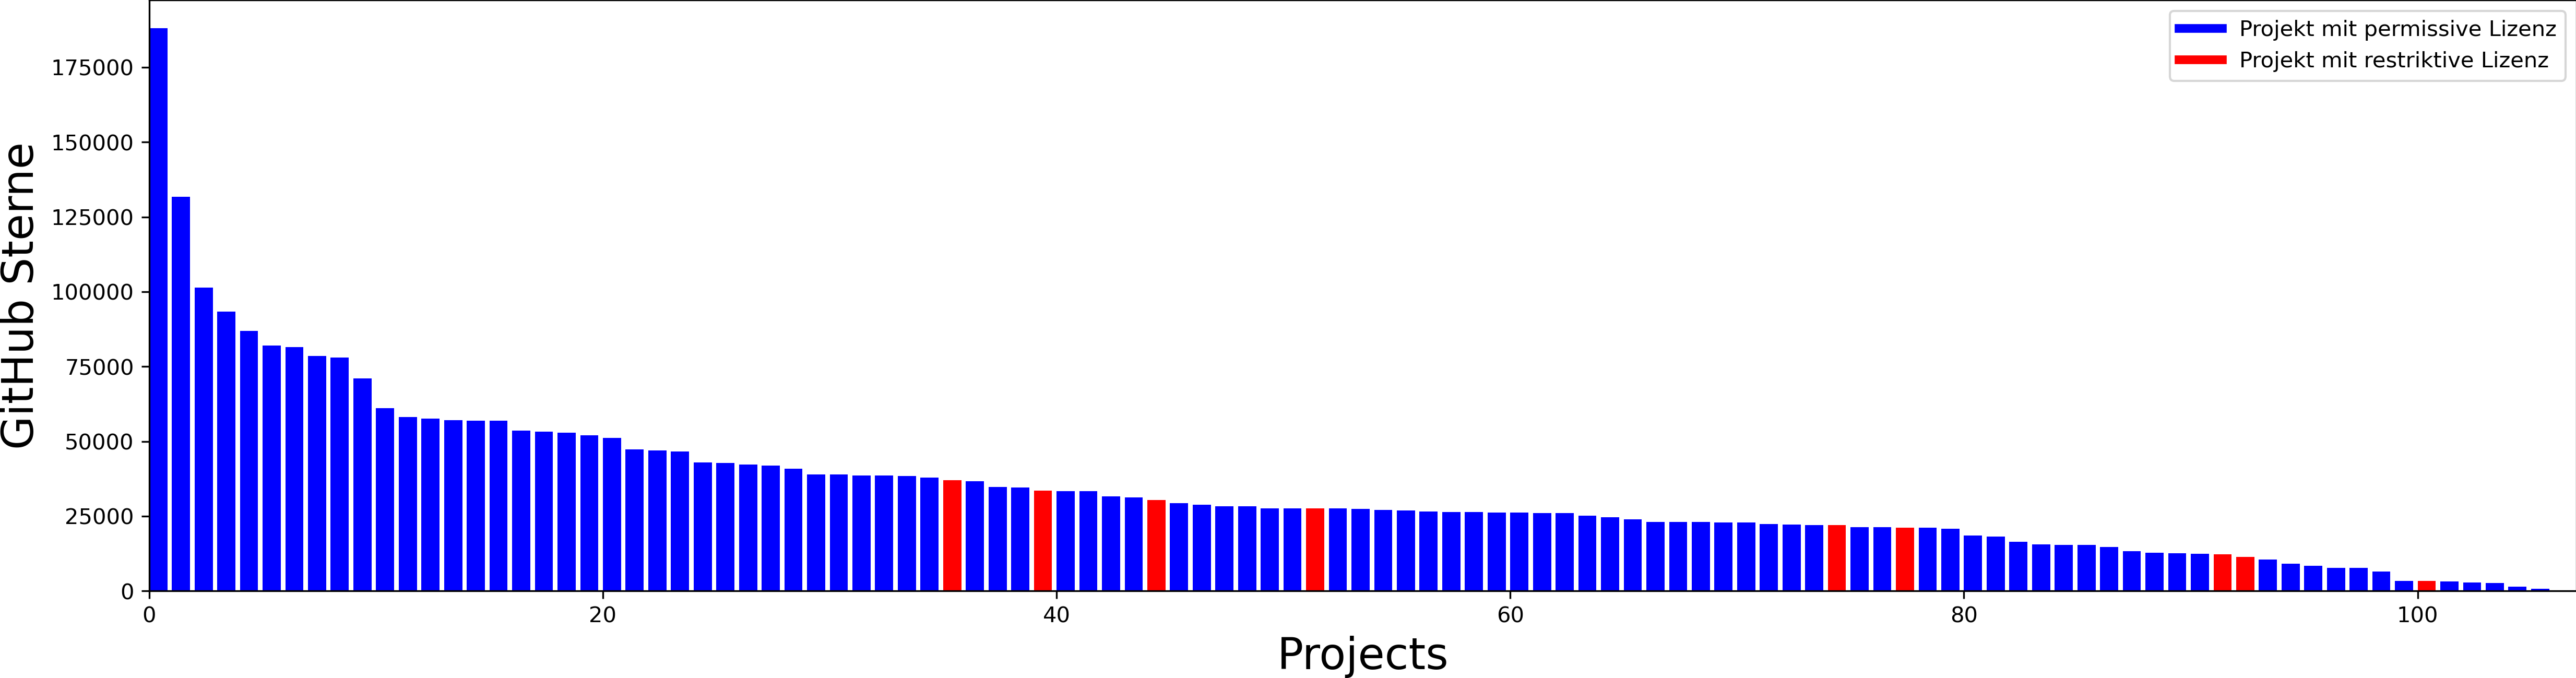
\includegraphics[scale=0.4]{figures/05/permissive_vs_restrictive_asBarChart.png}
    \caption{Effekt von Lizenzen auf GitHub Sterne}
    \label{abb:permissive_vs_restriktiv_BarChart}
\end{figure}

% Abbildung: Lizenzen vs Commits
\begin{figure}[]
    \centering
    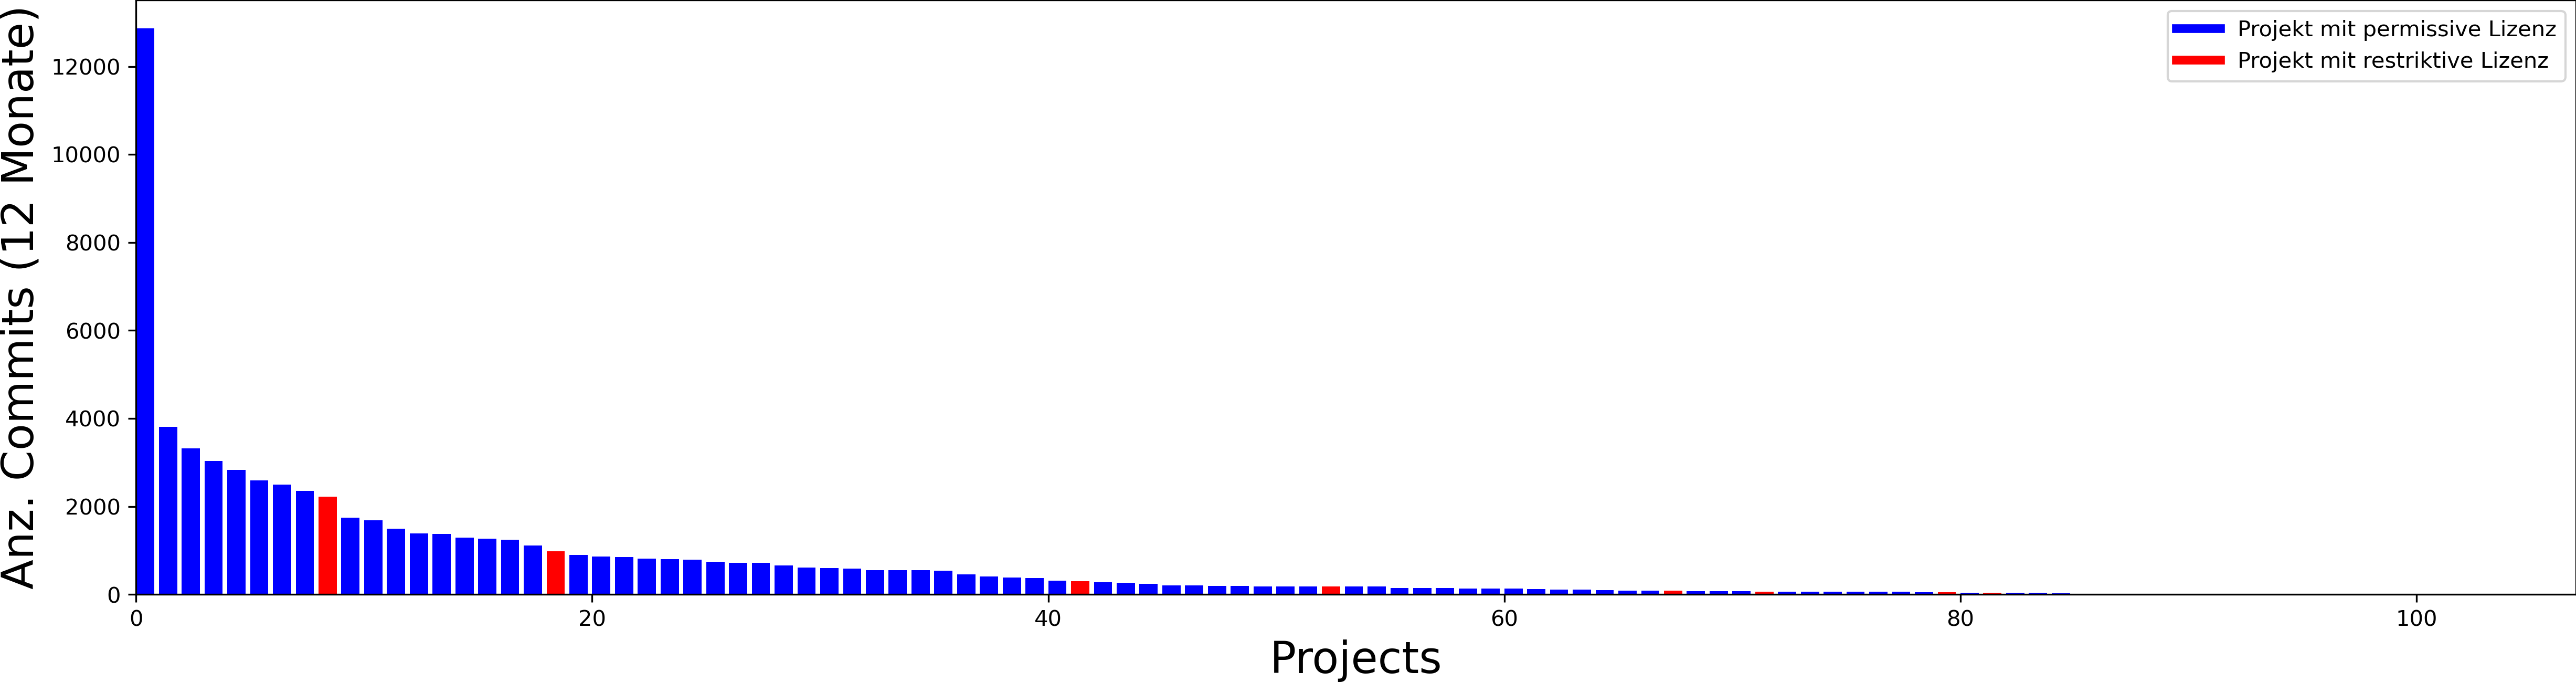
\includegraphics[scale=0.4]{figures/05/license_vs_last12MonthsCommits_asBarChart.png}
    \caption{Effekt von Lizenzen auf Anzahl der Commits}
    \label{abb:license_vs_commits}
\end{figure}



% ---------------------------------------- Code of Conduct --------------------------------------- %
\newpage %! newpage
\section{Code of Conduct}\label{sec:CoC}
Der Datensatz wurde hier erneut in zwei Gruppen geteilt, Projekte mit Code of Conduct und Projekte
ohne. Verglichen wurden GitHub Sterne und Downloadzahlen mittels Median. Der Median wurde in diesem
Fall gewählt, da sowohl Sterne als auch Downloads starke Ausreißer haben. Da nicht alle Projekte auf
NPM gelistet sind, beispielsweise Applikationen, wurden diese bei der Berechnung des Medians der
Downloadzahlen nicht berücksichtigt. So bildet sich der Median der Sterne aus 108  Datensätzen
und der Median der Downloads aus 88 Datensätzen.

Wie man in Tabelle \ref{tab:relation_CoC_Popularity} zu erkennen ist haben 53\% der Projekte einen
Code of Conduct.
Projekte mit Code of Conduct haben 51\% mehr Downloads auf NPM und 55\% mehr Github Sterne.
Da Projekte mit einem Code of Conduct beliebter sind, als die ohne bestätigt sich somit
\hyperref[H:4]{Hypothese H4}


\begin{table}[h]
    \begin{tabular}{l|c|c|}
        \cline{2-3}
                                  & \multicolumn{1}{l|}{\textbf{Projekte mit Code of Conduct}} & \multicolumn{1}{l|}{\textbf{Projekte ohne Code of Conduct}} \\ \hline
        \textbf{Anzahl}           & 57                                                         & 51                                                          \\ \hline
        \textbf{Median Sterne}    & 34.581                                                     & 22.279                                                      \\ \hline
        \textbf{Median Downloads} & 1.636.148,5                                                & 1.078.509,5                                                 \\ \cline{2-3}
    \end{tabular}%
    \caption{Relation von Code of Conduct und Beliebtheit}
    \label{tab:relation_CoC_Popularity}
\end{table}


% \begin{figure}[h]
%     \centering
%     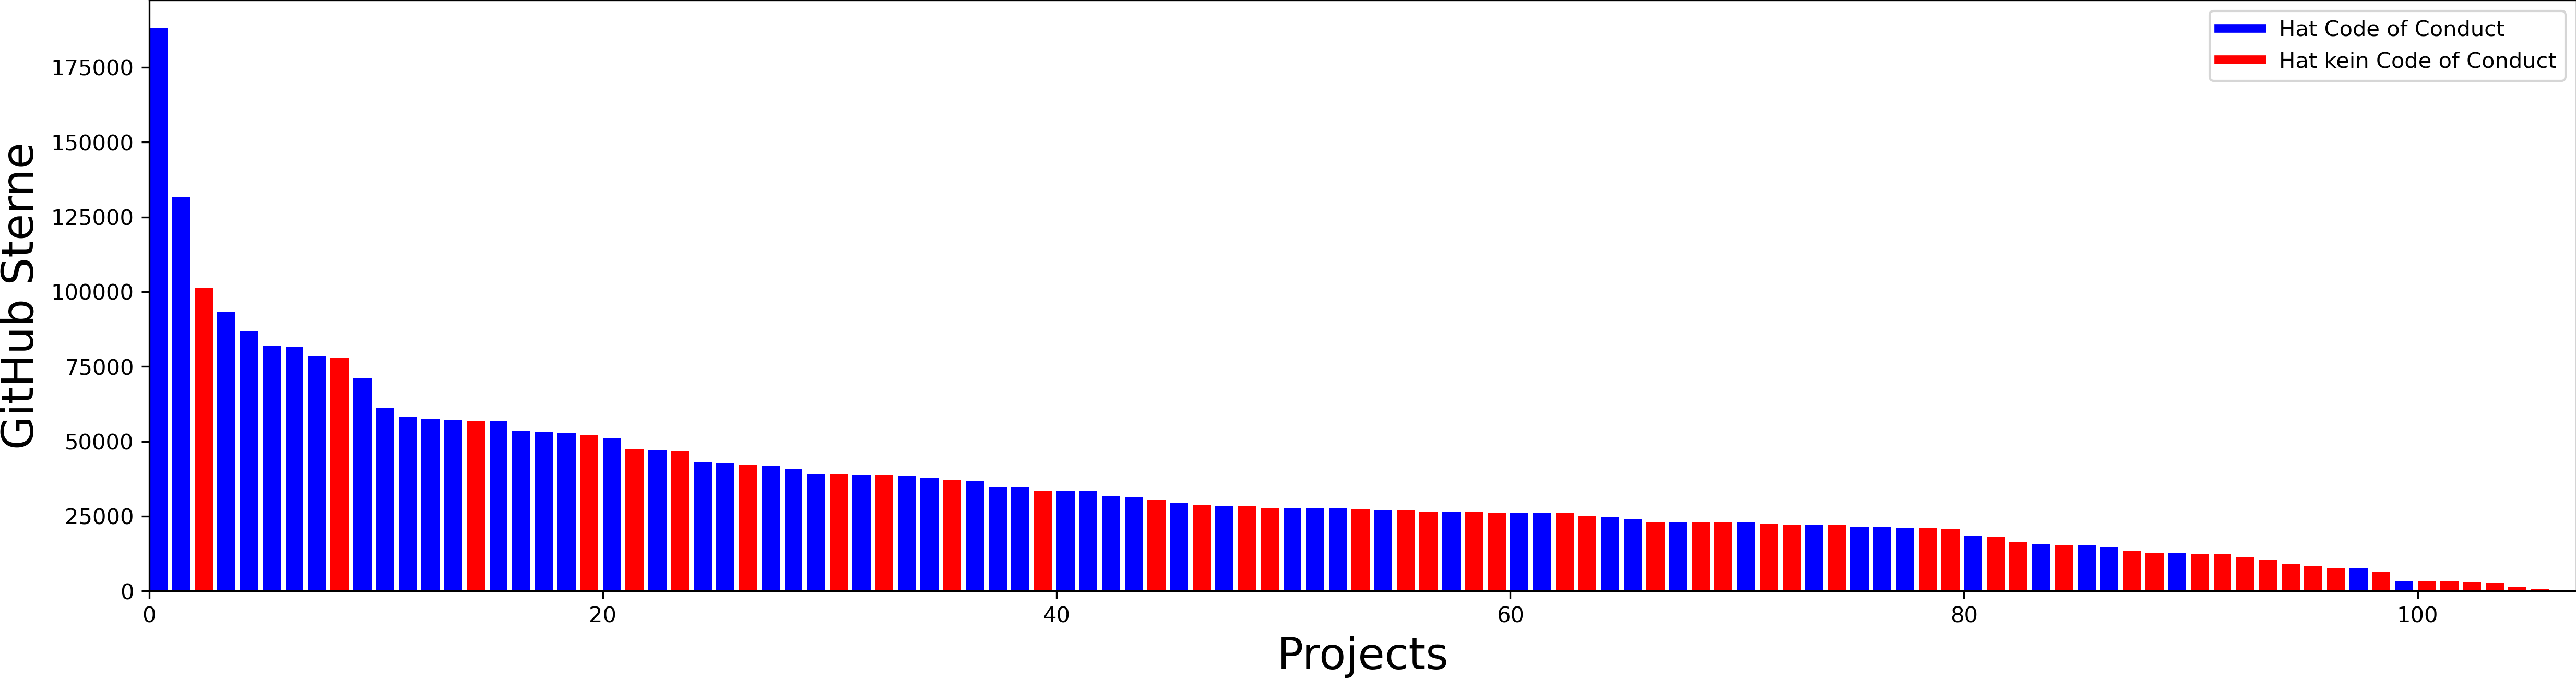
\includegraphics[scale=0.42]{figures/05/Stars_vs_CoC_asBarChart.png}
%     \caption{Einfluss von Code of Conduct auf Sterne}
%     \label{abb:CodeOfConduct_Stars}
% \end{figure}



% -------------------------------------- Contributing Guide -------------------------------------- %
\section{Contributing Guide}

\todo{Bonus Formulierung: Die Projekte die ein CG haben befinden sich in den Top 50\%....}

Wie im Kapitel \ref{sec:CoC} wurde auch hier der Datensatz in zwei Gruppen unterteilt. Projekte mit
und ohne einen Contributing Guide (CG). Hier soll der Zusammenhang zwischen dem Vorhandensein eines
CG und Anzahl der Contributor bzw. Commits \todoo{erforscht} werden.

Hierbei beschränken sich die Anzahl der Commits auf die letzten 12 Monate, um eine vergleichbare
Basis zu schaffen. Gleiches war bei den Contributor nicht umsetzbar, da die GitHub API keinen
Endpoint hierfür hat, somit werden Contributor über den gesamten Zeitraum des Projektes verglichen.

Anders als beim Code of Conduct, haben hier 86\% aller Projekte einen (CG).
In Abbildung \ref{abb:ContributingGuide_vs_Contributors} werden die Projekte nach Anzahl der Contributor
sortiert, wie man erkennen kann haben die Projekte mit den meisten Mitwirkenden alle einen CG. Das
erste Projekt ohne belegt hier Platz 54. Nach dem gleichen Schema wurden auch nach Anzahl der Commits
sortiert, das erste Projekt ohne CG landet hier auf Platz 42.

In beiden vergleichen platzieren sich Projekte mit CG weit vor Projekten ohne. Wie in \hyperref[H:5]
{Hypothese H5} angenommen hat der Contributing Guide einen positiven Effekt auf den technischen Erfolg.

\begin{figure}[h]
    \centering
    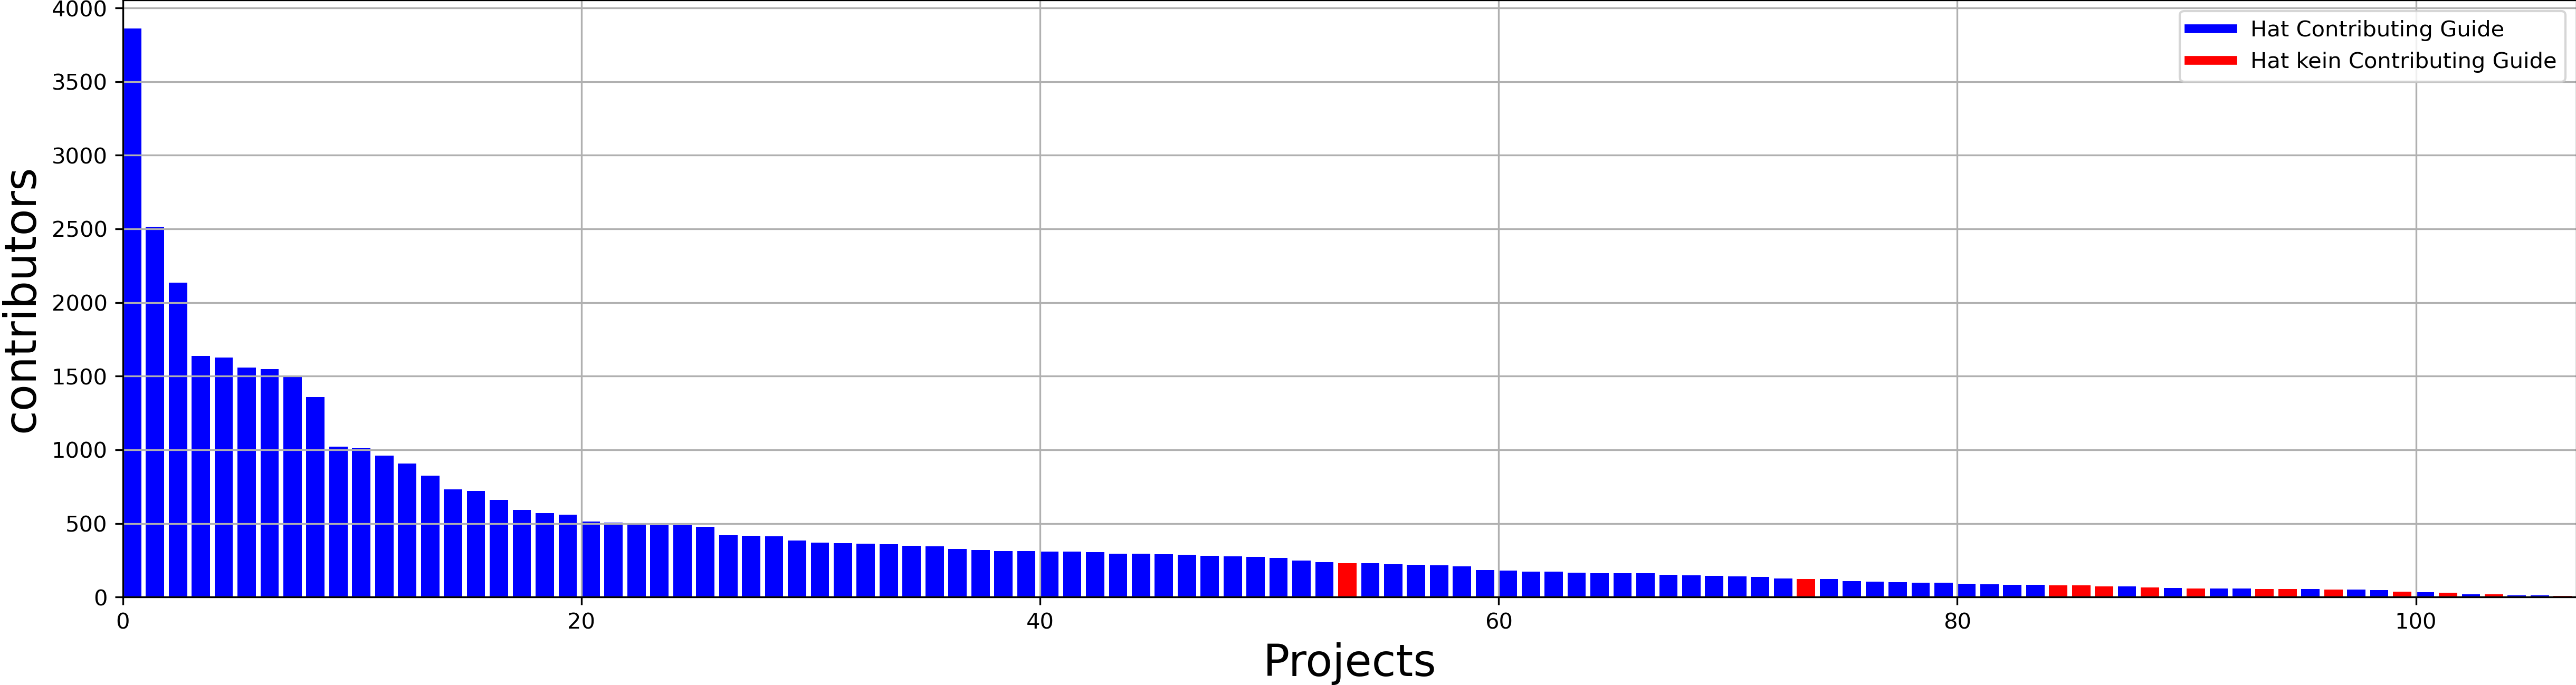
\includegraphics[scale=0.42]{figures/05/Contributors_Projects_asBarChart.png}
    \caption{Einfluss von Contributing Guide auf Contributor}
    \label{abb:ContributingGuide_vs_Contributors}
\end{figure}

\newpage %! new Page
\section{Einfluss von Sponsoren auf den technischen Erfolg}

Erneut wurde der Datensatz in zwei Gruppen geteilt, Projekte mit und ohne Sponsoren. Verglichen wurde
der Median der Commits der letzten 12 Monate sowie die Anzahl an Contributor. In Tabelle \ref{}

\begin{table}[h]
    \begin{tabular}{l|c|c|}
        \cline{2-3}
                                                      & \multicolumn{1}{l|}{\textbf{Projekte mit Sponsoren}} & \multicolumn{1}{l|}{\textbf{Projekte ohne Sponsoren}} \\ \hline
        \textbf{Anzahl der Projekte}                  & 56                                                   & 52                                                    \\ \hline
        \textbf{Median Anz. Sterne}                   & 26.468                                               & 27.551                                                \\ \hline
        \textbf{Median Anz. Downloads}                & 1.409.792                                            & 1.094.063                                             \\ \hline
        \textbf{Median Commits der letzten 12 Monate} & 221                                                  & 128                                                   \\ \hline
        \textbf{Median Anz. Contributor}              & 289                                                  & 155                                                   \\ \hline
    \end{tabular}%
    \caption{Relation von Sponsoren und Erfolg}
    \label{tab:Sponsors_vs_NonSponsors}
\end{table}

- Bisschen Tricky weil manche keinen Sponsor haben aber dafür von Unternehmen her aus kommen.\\
- Hier könnte man die Hypothese ändern auf "Finaziell unterstützte Projekte sind erfolgreicher"
dann schließt man nämlich auch die Unternehmen und Foundations mit ein und dann easy. Dann fasst man einfach
Sponsor == 1 mit, BackedBy == 1, BackedBy == 2 zusammen und gute Nacht. Hier wird es evtl möglich sein
wieder mit Median etc zu arbeiten, je nachdem wie spread die daten sind.